\begin{figure*}[t!]
\centering
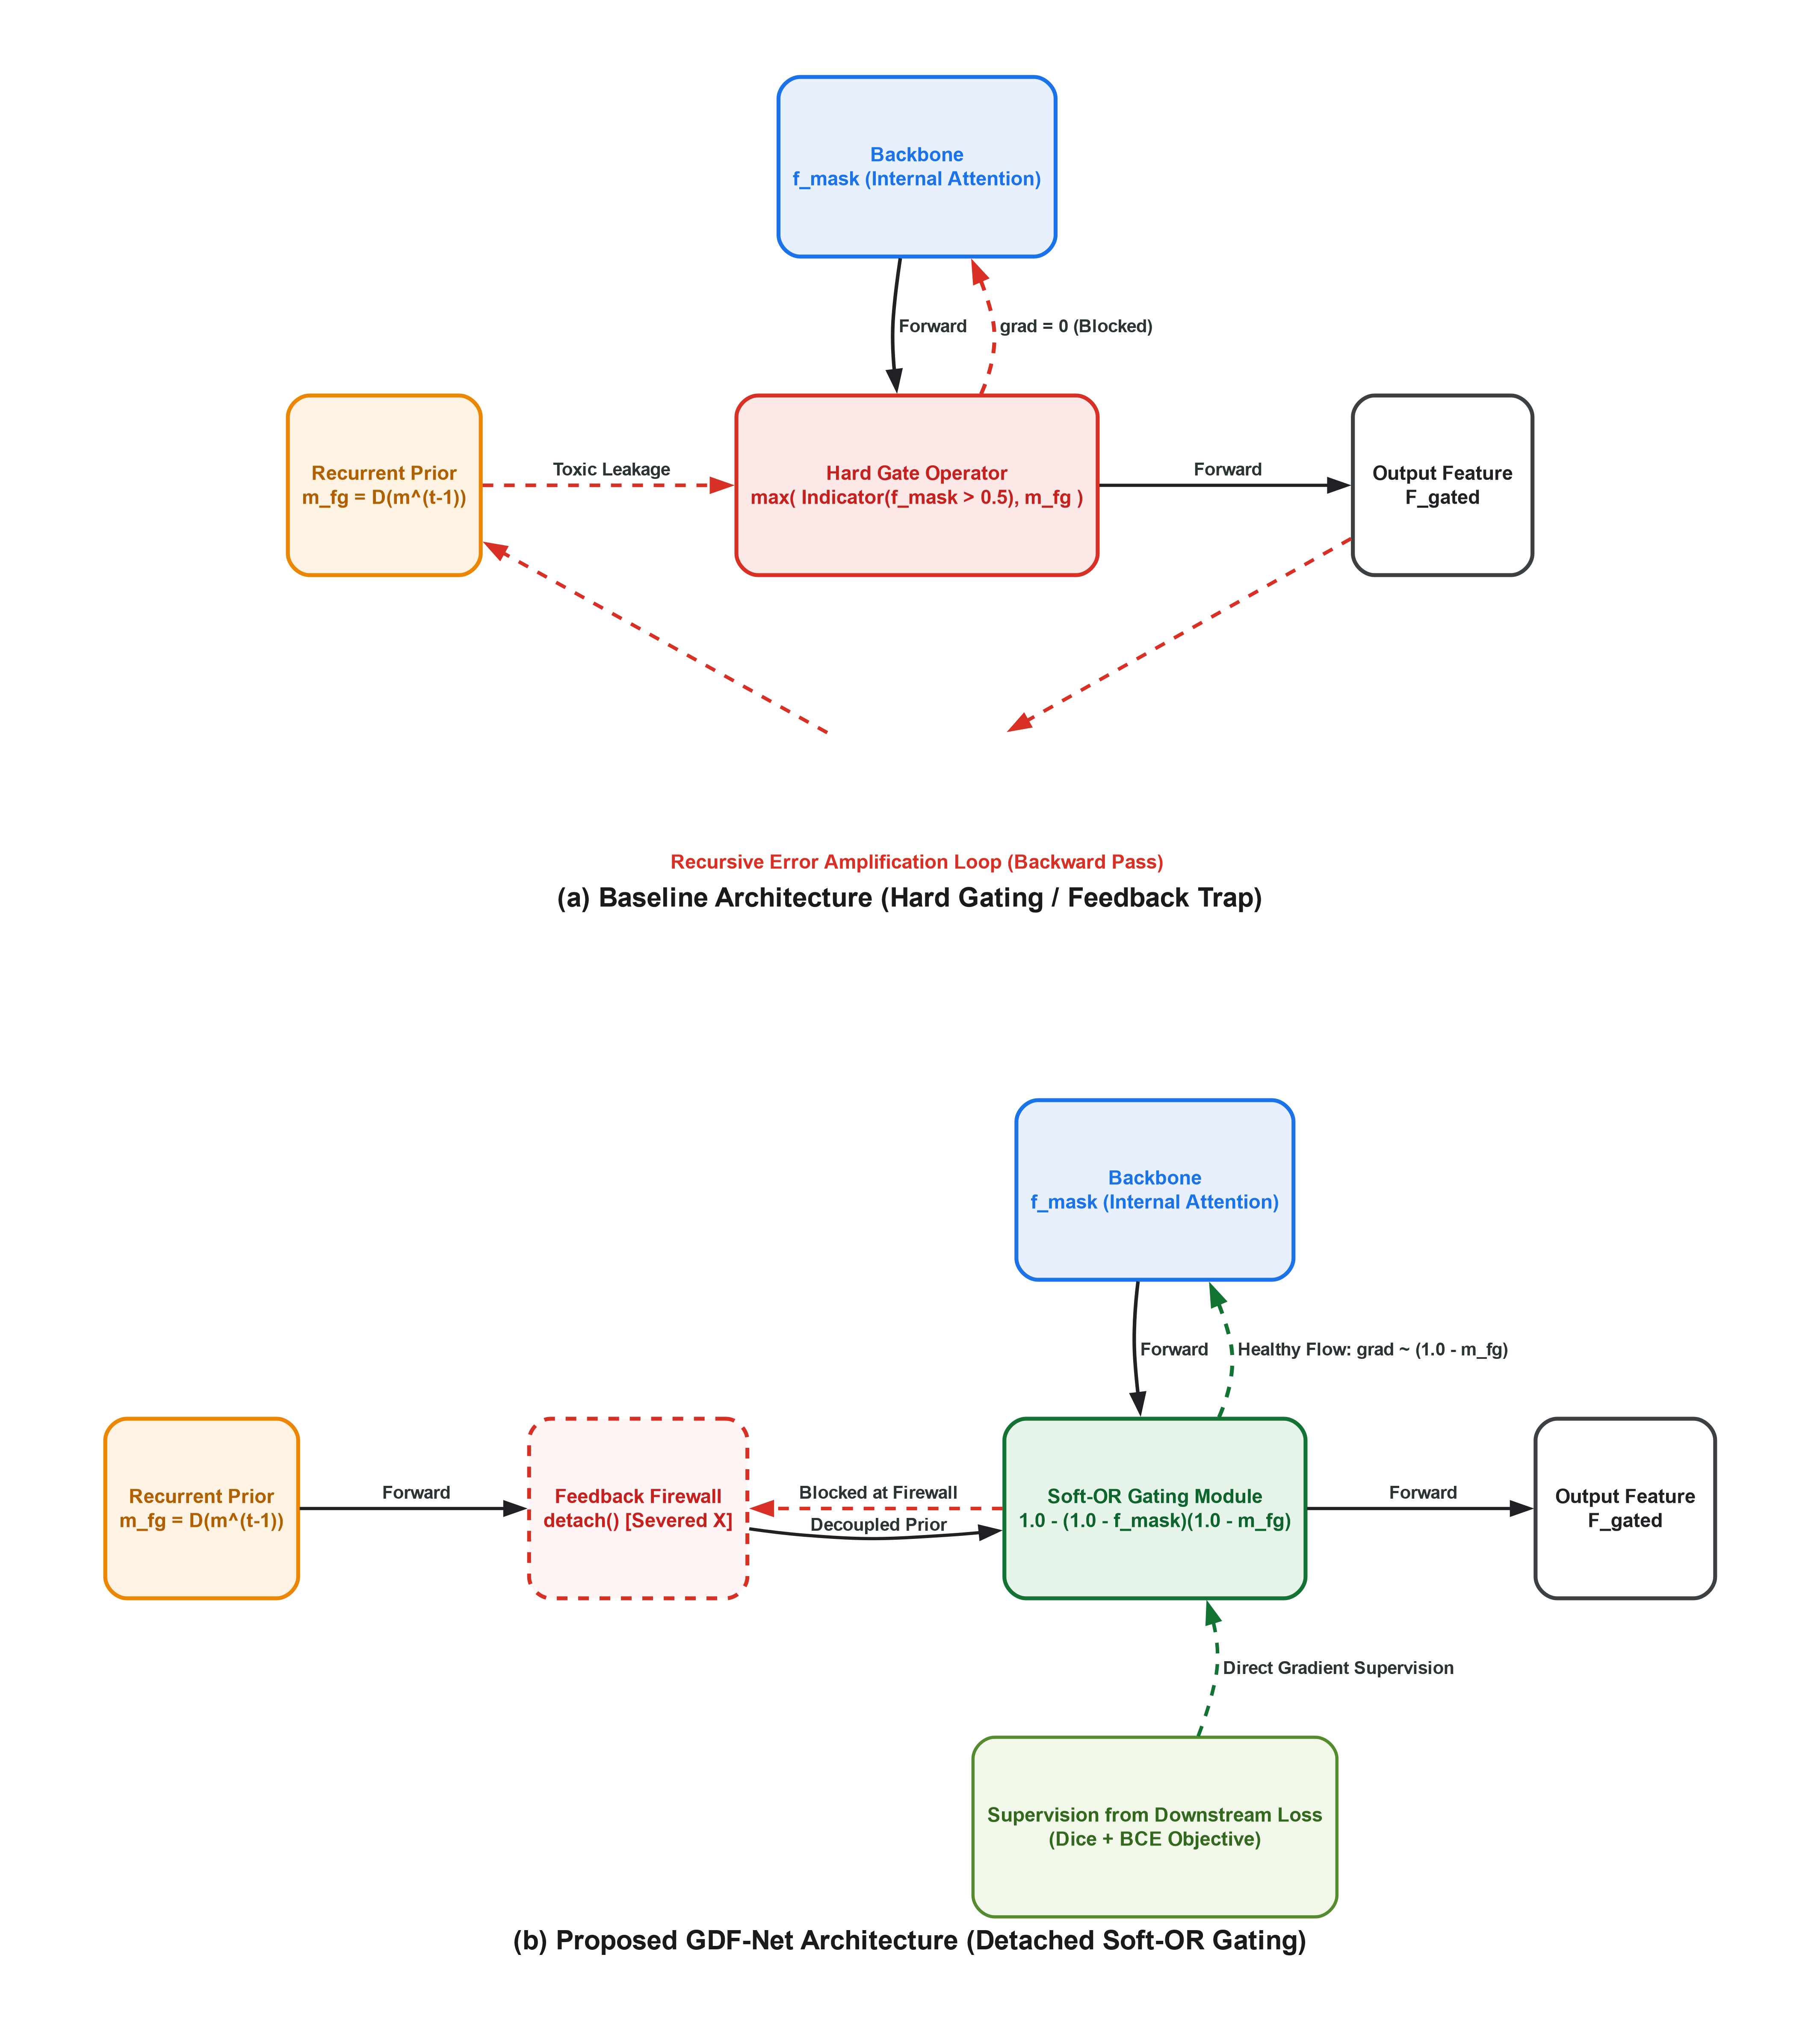
\includegraphics[width=0.92\textwidth]{figures/architecture_diagram.png}
\caption{Architectural comparison of spatial feedback gating mechanisms rendered via Diagram as Code (\texttt{mingrammer/diagrams}). Solid black arrows denote forward feature propagation; dashed colored arrows represent backward gradient backpropagation. \textbf{(a) Baseline Architecture (Hard Gating / Feedback Trap):} Step-function gating induces gradient paralysis on internal attention ($\text{grad} = 0$), while toxic recursive error leaks into the recurrent prior, causing irreversible false-positive over-segmentation. \textbf{(b) Proposed GDF-Net Architecture (Detached Soft-OR Gating):} The Feedback Firewall (\texttt{detach}) mathematically severs recursive gradient backpropagation while continuous Soft-OR modulation restores dense, uncertainty-guided gradient backpropagation.}
\label{fig:architecture_diagram}
\end{figure*}
